\documentclass[border=0pt]{standalone}
\usepackage{tikz}
\usepackage{graphicx}
\usetikzlibrary{decorations.markings, decorations.pathmorphing, arrows.meta, calc}
\usetikzlibrary{decorations.pathreplacing, arrows.meta}
\usepackage[dvipsnames]{xcolor} % Use colors from dvipsnames

\begin{document}
\begin{tikzpicture}
	% Include the first image (PDF)
	% should only be blue points to work well
	\node[anchor=west,inner sep=0, outer sep=0] (img1) at (0,0)
	{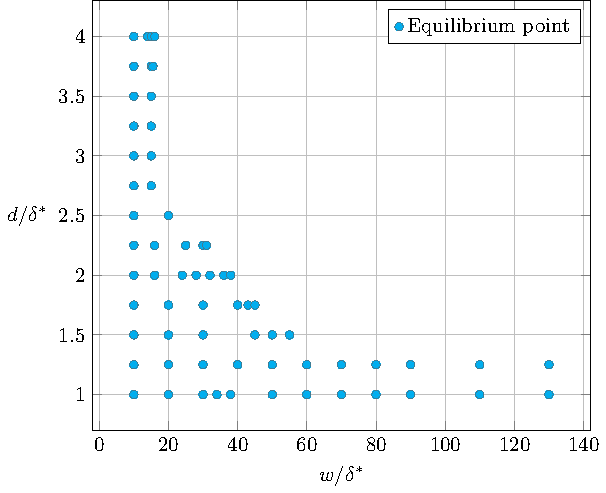
\includegraphics[width=5cm]{incNS2dStabilityCurve_equilibria.pdf}};

	% Include the second image (JPG), to the right of the first
	\fboxsep=0pt % Remove extra padding inside the frame
	% fbox color
	\node[anchor=west,inner sep=0, outer sep=0] (img2) at ([xshift=0.0cm]img1.east)
	{\fcolorbox{Cyan}{White}{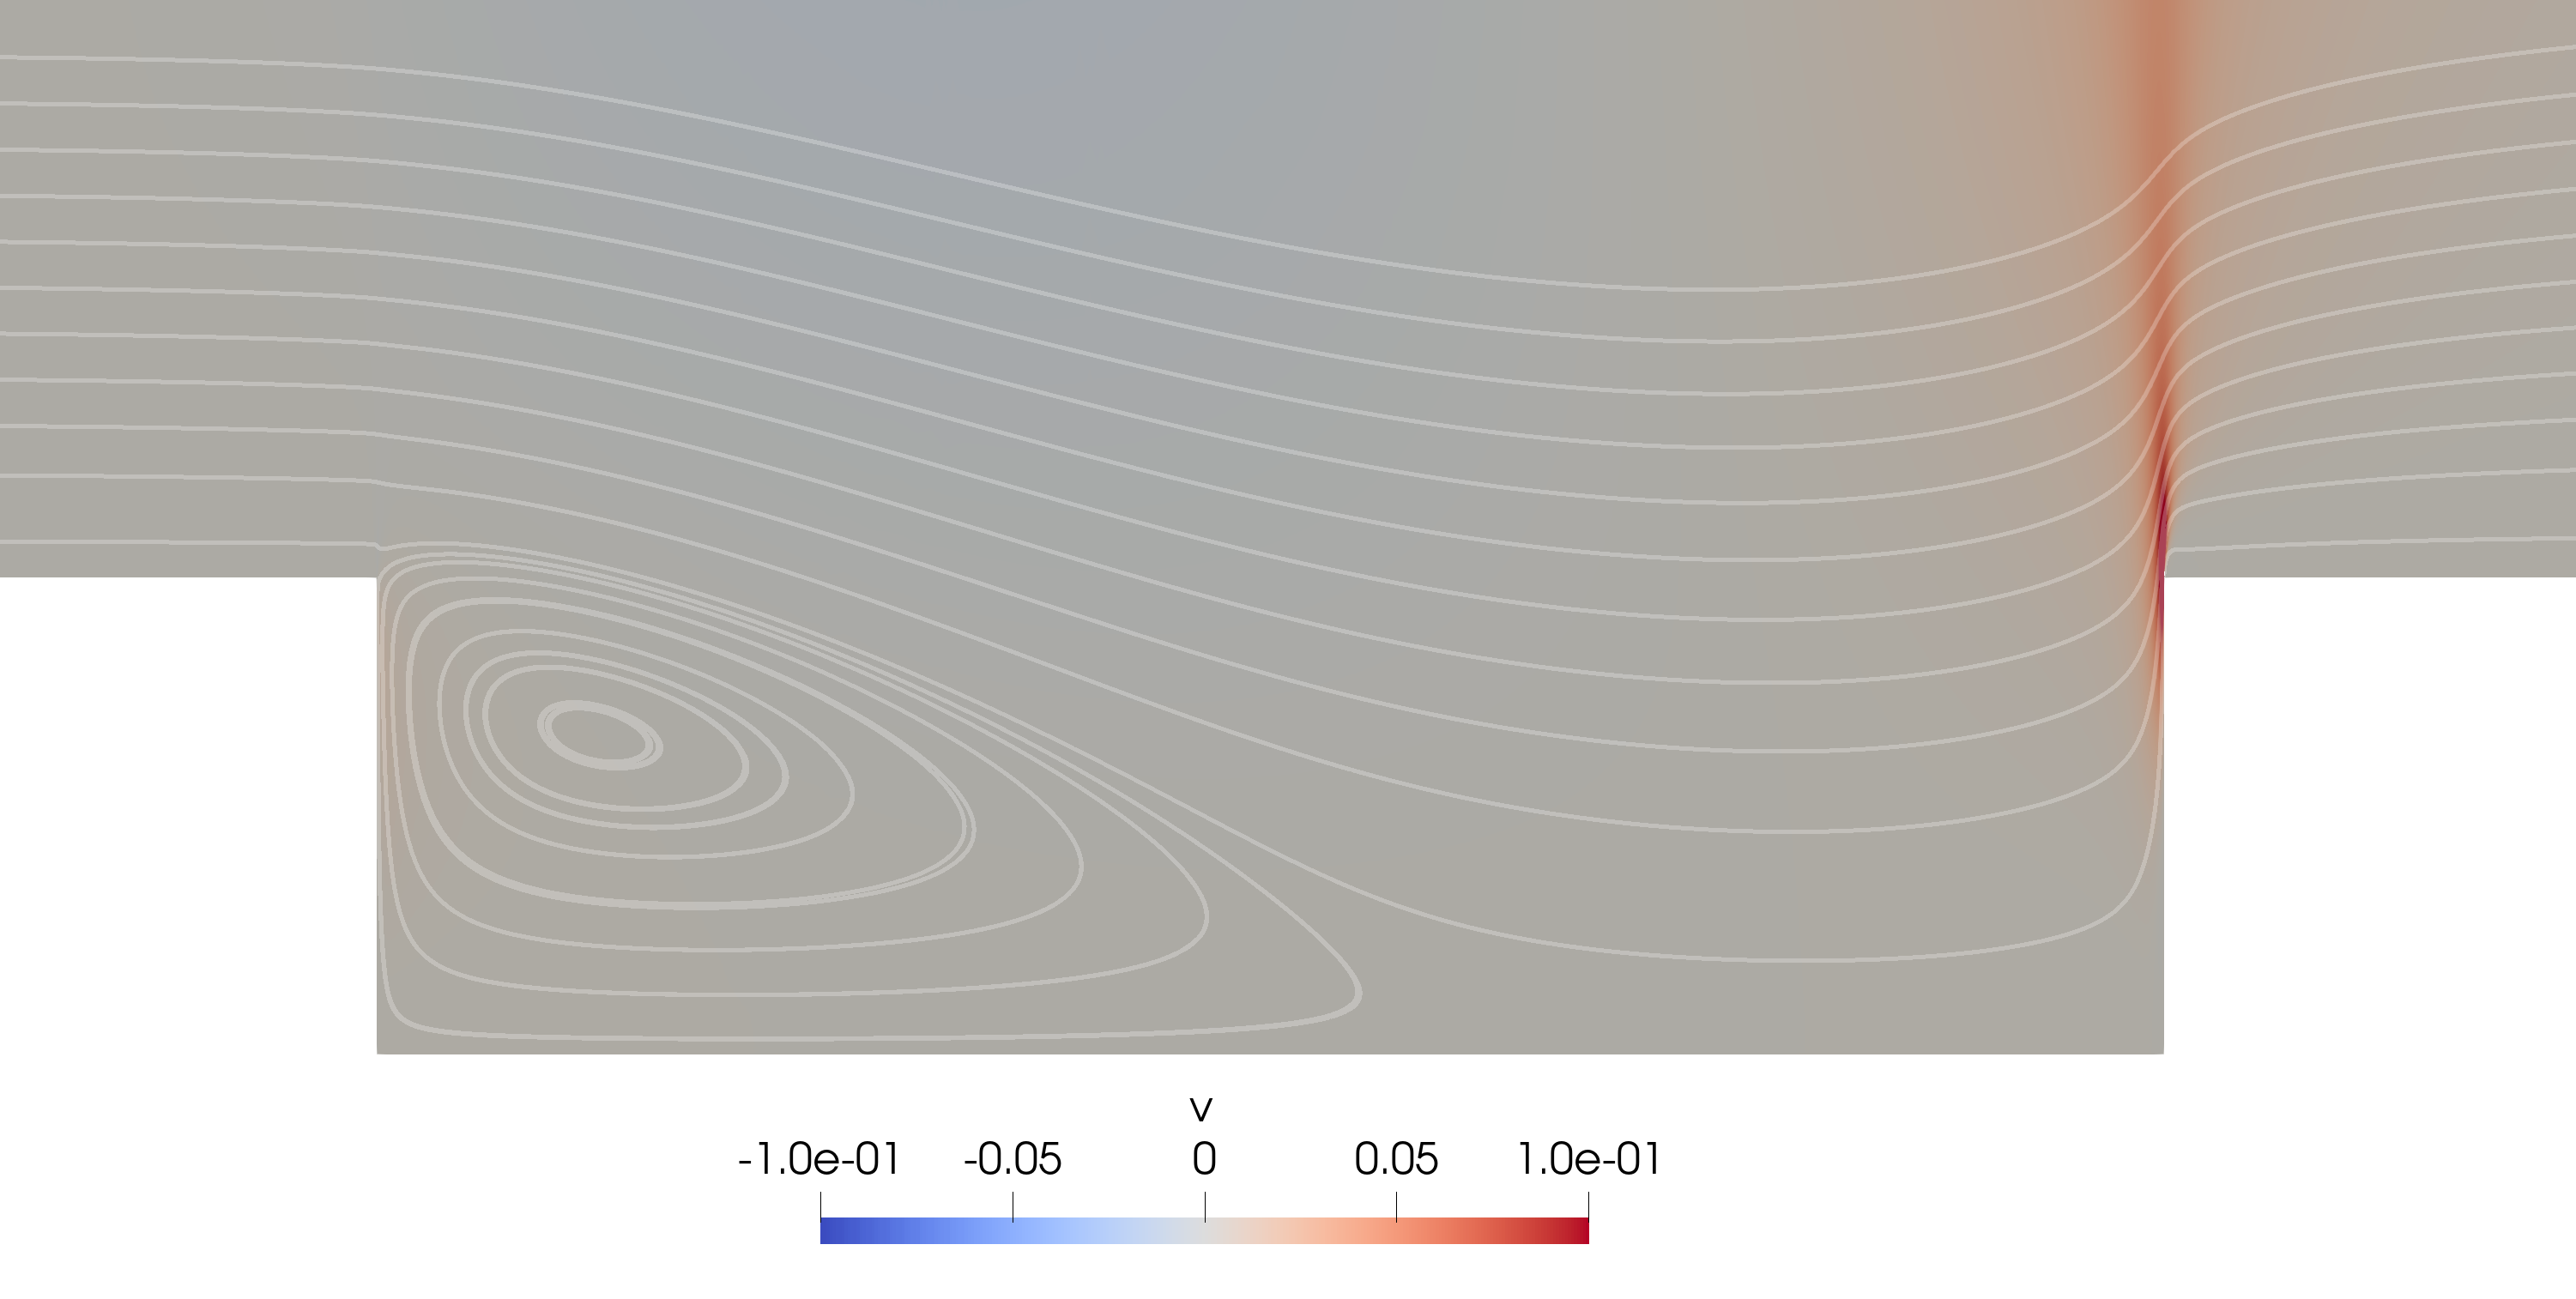
\includegraphics[width=5cm]{../../../Images/d1_w60_streamlines.png}}};

	\node[anchor=north,inner sep=0, outer sep=0] (img3) at ([yshift=-0.05cm]img2.north){\fcolorbox{black}{white}{
\includegraphics[width=1.5cm]{../../../Images/d1_w60_real.png}}};

	\node[anchor=south,inner sep=0, outer sep=0] at ([yshift=0.4cm]img2.north) {$d/\delta^* = 1,\quad w/\delta^* = 60$};

	% % Draw arrow from center of first image to center of second
	\draw[
	  line width=0.5pt,       % thin line
	  Cyan,
	] 
	(2.52,-1.22) -- ([xshift=0.01cm,yshift=-0.01cm]img2.north west);

	\draw[
	  line width=0.5pt,       % thin line
	  Cyan,
	] 
	(2.52,-1.23) -- ([xshift=0.01cm,yshift=0.01cm]img2.south west);


\end{tikzpicture}
\end{document}
